%\part{State of the Art}

\part{Optimization}

\chapter{Basic Concepts}

Before starting to present the different categories of optimization, we would like to take some time defining what exactly optimization is.\\
In the more general way, optimizing is \emph{trying to find the best element among an element set}. When finding this best element is not trivial, we can rightfully talk of \emph{solving an optimization problem}. This seemingly simple definition implies in fact quite a lot.

First of all it requires we have a defined set of element to choose from. As we will see, the topology of the set is of the utmost importance for choosing the way of solving the problem. This set of element is often named the \emph{search space}, \emph{solution space} or \emph{domain}. In "simple" optimization problems, the search space can be simply defined by a set of elements (for example \{a,b,c\} or \ensuremath{\mathbb{R}}) associated with a set of \emph{constraints}. For large problems, the search space can be defined by calculus-heavy equations, empirical models, complex algorithms ... or even a mix of all of the above.

\definition{Search space}{the set containing all the possible candidates of the optimization problem.}

While we said that the search space can be defined by a set of constraints, it is often more convenient to express the constraints separately. For example, if the search space of an optimization problem is defined over all the real numbers lower than 2, instead of defining the search space as [-\(\infty\) : 2], it will usually be refereed as \(\mathbb{R}\), with the added constraint \(x < 2\). Usually we say the problem to be \emph{subject to (s. t.)} the constraint \(x < 2\).\\
In theory these two formulations should be equivalent. In practice however, these constraints are often the result of a real-world concern, and thus subject to some inherent imprecision. [[WHAT ?? THE TRAVEL IS INTRODUCED AFTER]] Back to our travel metaphor, we can imagine that we set the maximum travel cost we are ready pay to a price of one thousand euro. Does that really means that a solution which would cost one thousand euro \textbf{and one cent} would be unacceptable ? Obviously not.  In engineering design, this is a common situation, and making these constraints explicits can be advantageous.

Since we want to find the best element of this solution space, we have to determine what make an element better than another. Usually, the possible solutions are compared through a specific function called the \emph{objective function}. Some alternate names are \emph{criterion} or \emph{cost function}. The best element would be the one for which the objective function returns a minimal (or alternatively, maximal\footnote{Obviously we sometimes want to find the \emph{maximal} value which is solution of a problem, however minimizing f(x) is equivalent to maximizing (-f(x)). So maximization problems can be expressed as minimization problems, and vice-versa. Traditionally, optimization problems are often expressed in the terms of finding a \emph{minimal} value since the two possibilities are equivalents.}) value. It should be noted that it is possible for a problem to admit several equivalent solutions in regard of the objective function.

\definition{Objective function}{a function defined over the search space of the optimization problems.}

The least obvious keyword here is \emph{try}. When the search space is very large, or its topology is complicated, it can be really long or difficult to find the best solution and, more important, to be sure that the solution is the best. In fact, in these problems, the only way to find the best solution with certainty is an exhaustive exploration of the search space. Since it can be very costly in terms
of time and calculation, instead of finding the best solution, we settle for a solution which is "good enough", for example because this solution is the best for a subpart of the search space. The best solution is called the \emph{global optimum}, while a "good enough" solution is called a \emph{local optimum}. In a similar fashion, methods which try to find the global solution are said to be \emph{global optimization methods}, where methods which search for local optimum are said to be \emph{local optimization methods}.

\definition{Optimizing}{finding an element of the search space which minimize (or maximize) the value of the objective-function}

\begin{figure}
\centering
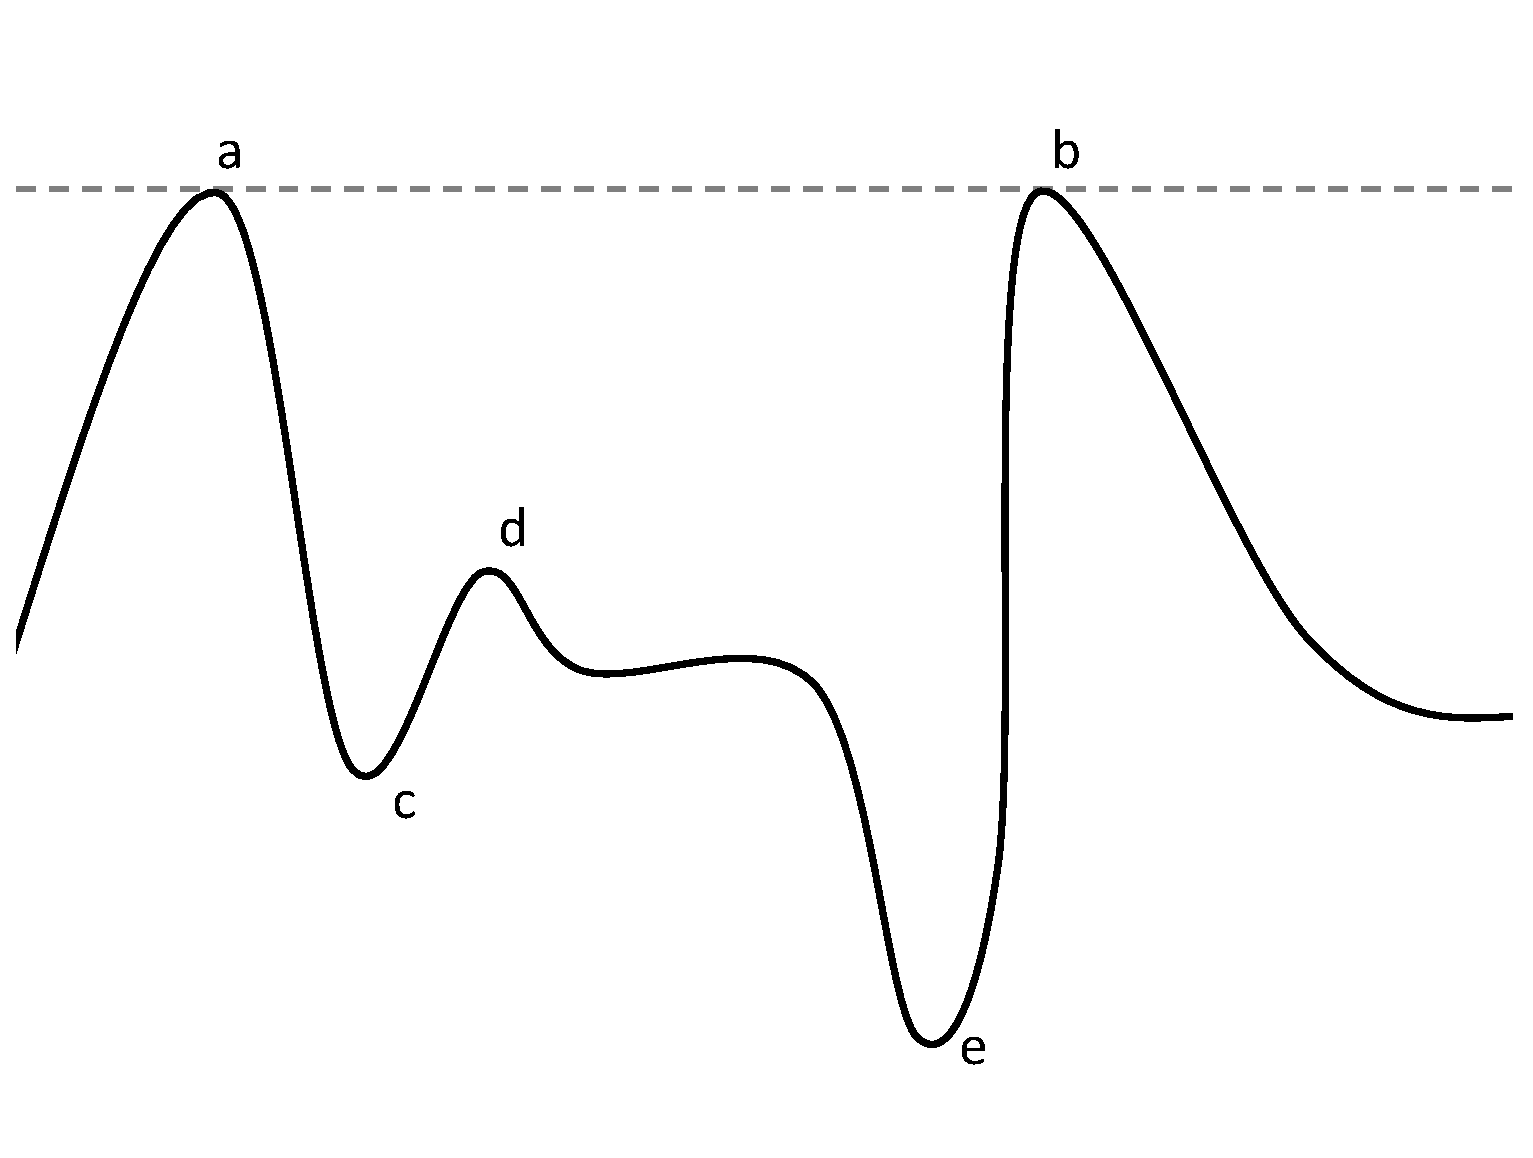
\includegraphics[width=0.4\paperwidth]{searchSpace}
\caption{Examples of local and global optimums.}
\label{localAndGlobalOptims}
\end{figure}

In figure \ref{localAndGlobalOptims}, we can see different examples of global and local optimums. The points labeled \emph{a} and \emph{b} are both global maximums, as they have the same value. The points
\emph{c} and \emph{d} are respectively local minimum and maximum, while \emph{e} is the global minimum.

From all the preceding, we can provide the minimal formulation of an optimization problem as follow 

\definition{Optimization problem}{
\begin{align*}
\text{minimize } &f(x) \\
\text{subject to } &(x \in S)
\end{align*}
Where \emph{S} is the problem search space and \emph{f(x)} the objective function.}

\section{No Free Lunch Theorem}
[[AVANT OU APRES LA DESCRIPTION DES DIFFERENTES METHODES ?]]

[[Compromis entre Exploration et Exploitation cf Berro Thesis]]

\section{Numerical versus Combinatorial Optimization}

\chapter{Numerical Optimization}

A great variety of methods exits in the literature. These methods can be segregated by the type of problems they aim to solve or some inherent properties of the method.

Some possible criteria to discriminate based on the type of problem:
\begin{itemize}
\item is the problem constrained ?
\item is the problem linear (or possibly quadratic) ?
\item is the problem convex ?
\end{itemize}

For the method in itself:
\begin{itemize}
\item does the method provides a global solution or a local one ?
\item does the method use derivatives ?
\item is the method deterministic or stochastic
\end{itemize}

\section{Local Methods}

\subsection{Linear}

[[simplex]]

\subsection{Using Derivatives}

[[
Gradient decent

Convex Hull

Simplex

SQP
]]

\subsection{Derivative-Free}

[[
Nelder Mead Simplex

Interpolation model
]]

\section{Global Method}

\subsection{Deterministic}

[[
Branch and Bound

Taboo search
]]

\subsection{Stochastic}

[[
Simulated Annealing

Monte-Carlo
]]



\subsection{Deterministic Methods}

\subsection{Stochastic Methods}

\chapter{Multi-Objective Optimization}

Multi-objective optimization (MOO) departs significantly from previous categories of optimization in the fact that you have to consider multiple objective functions instead of one. A main aspect of MOO is the way to conciliate these objectives, which are usually contradictory.
An example of real-world everyday MOO problem could be choosing the mean of transportation for a travel, trying to find a balance between speed and cost. Airplane is the fastest way of transportation, but is expensive. While car is slower, it is cheaper. Train is slower than plane, more expensive than car, but can preferred as the best compromise. There still, however, are solutions which are strictly worse than others (in our example, renting an helicopter would probably be both more expensive and slower than buying a seat on a commercial airplane).
From this example we can see that, for a MOO problem, there rarely is a clear-cut "best" solution. And more importantly that even some solutions which are not optimum for \emph{any} of the objectives can be deemed satisfying. Only when each objective is completely independent, or when no objective is contradictory to another, then a MOO problem can be handled as a set of separated mono-objective optimization problems.
A solution vector which would be optimum for each objective is sometimes called \emph{utopia point}, or \emph{shadow minimum}, and is used as a reference comparison in some of the MOO techniques we present.

[[FORMULATION OF A MOO PROBLEM]]

MOO problems are quite a radical departure from previous optimization problems type we have seen. Many approaches have proposed, the majority of which can be separated in to categories: \emph{a priori} and \emph{a posteriori} approaches. A priori approaches aims to discriminate between the objectives \emph{before} the optimization process. This often consist into combining the different objectives into one, before applying a classical optimization method on the new, aggregated objective.
On the opposite, a posteriori methods tries to provide a set of efficient solutions among which the decider will choose.
A priori approaches are considered easier, but not very efficient, whereas a posteriori approaches provides more diversity of solutions as well as more insight about the nature of the problem.
A third category can also be considered: the \emph{interactive} methods. Basically, these methods iterates between decision and search phases. For example, an interactive  method could work by quickly providing intermediate solutions to the decision-maker, which would in return refine the search using them.

We will now see some of the strategies have been proposed to deal with such a type of problem.

\section{A Priori Methods}

\subsection{Objectives Aggregation}

The first approach is to transform the MOO problem back to a mono-objective optimization problem, by aggregating the different objectives into one. This can be expressed as follow : \(f_g = aggr(f_1, f_2, ..., f_n)\), where \(f_1, f_2, ..., f_n\) are the original objectives and \(f_g\) the aggregated one, which will be used with classical mono-objective optimization methods.

Concerning the choice of the aggregation function, different strategies can be used.

Concerning the choice of the aggregation function, the simplest strategy is to use a classical function such as addition, multiplication, mean, max or min of the objectives, and variations of the preceding (exponential sum, ...): these methods present the major drawback of requiring the aggregated values to be comparable.[[ Keeping with our travel example]], is it relevant to simply add duration and cost ?

A slightly more sophisticated way is to use pondered mean: we attribute a coefficient to each objective when adding them :

\[ f(x) =\sum_{i=1}^n w_i f_i(x) \]

Where $w_i$ are the coefficients representing the relative preferences between the objectives.

This method allows to express a preference between different objectives, as well as bringing back on comparable scale different objectives. However, one now has to decide of the coefficients to choose. Also, this method can hide some information concerning the solution, for example an extremely poor result in one of the objectives, compensated by small improvements in all the others.  [[Moreover, this solution present some limitations when the solution space is nonconvex [[EXPAND]]]]

[[To get refs which criticize Weighted sum, see "Survey of multi-objective optimization methods for engineering"]]

\subsection{Lexicographic Method}

In this method, the objectives functions are arranged and optimized by order of importance. The result of the optimization at a given step become a constraint to satisfy for the following steps.

Formally, the problem become an ordered set of optimization problems expressed as follow:

\begin{align*}
\text{min } &f_i(x) \\
\text{subject to } &f_j(x) \leq f_j(x_j^*) \\
j = &1, ..., i-1
\end{align*}

A variation of this method proposes to replace inequalities by equality constraints. [[REF]]

Another variation, sometimes called hierarchical, introduces a constraint relaxation coefficient $\delta$ where the new formulation of the constraints becomes:

\[ f_j(x) \leq \left(1 + \frac{\delta_j}{100}\right) f_j(x_j^*) \]

\subsection{$\epsilon$-constraint Method}

The $\epsilon$-constraint method proposes to change the expression of the problem by keeping only one objective (the one deemed the most important) and transforming the others into inequality constraints.

For example, the problem \[\text{min } f_1, f_2, ...,f_n\] where $f_1$ is deemed the most important objective would be transformed in
\begin{align*}
\text{min } &f_1 \\
\text{subject to } &f_2 \leq \epsilon_2, ..., f_n \leq \epsilon_n
\end{align*}

Where $\epsilon_2, ..., \epsilon_n$ must be chosen by the designer.
Depending of the selection of $\epsilon_2, ..., \epsilon_n$, it is possible to obtain a formulation where no feasible solution exist.
[["Survey of multi-objective optimization methods for engineering" -> Bounded objective function method for some ref about methods to select \epsilon]]

\subsection{Goal Programming}

[[REF in "Survey of multi-objective optimization methods for engineering"]]

The idea of Goal Programming (also called Target Vector Optimization) is to fix for each objective an associated goal to reach. Each objective can be over- or underachieving its goal, allowing the designer to provide a rough idea of the initial design goals.

The new objective is to minimize the total deviation $\sum_{i=1}^n |f_i - g_i|$ where $g_i$ is the goal associated to objective $f_i$.

Goal Programming is very easy to use and quite popular, and can work even when the designer provided some unreachable goals, but provides no guarantee for the optimality of the solution.

\subsection{Min-Max Method}

This method use the separately attainable minima of the objectives (the so-called \emph{utopia point}) and try to minimize the maximum deviation of the objectives relative to those minima:

\[ \text{min } f = \text{ max } \left( \frac{f_i - f_i^0}{f_i^0} \right) \]

where $f_i^0$ represent the separately attainable minimum of the objective $f_i$.

This method can also be used similarly to Goal Programming, where the separately attainable minima are replaced by goal given by the designer.

A variant of this method, called weighted min-max, or Tchebycheff method, use the following formulation:

\[ \text{min } f = \text{ max } w_i |f_i - f_i^0| \]

where $w_i$ are coefficient provided by the designer.

[[Talk of variants ??]]

\subsection{Analysis of a priori methods}

A priori methods provide a simple and efficient way to tackle the problem of multiple objectives, as they allow to reduce the problem to a mono-objective one.
However, a drawback of these methods is the need for the designer to have a good knowledge of the problem, to know the correct way to combine/compare the different objectives functions. In the general case, the designer could not have enough experience or information to make such decision.

In the case where the designer would have enough knowledge to meaningfully use such a method, the introduction of this knowledge can risk to introduce a bias in the resulting solution, orienting the optimization process toward "standard" solutions at the expense of possible non-conventional ones.

Moreover, aggregations techniques tend to break when the objectives are not comparable, requiring once more knowledge from the designer to introduce adjustment coefficients to re-equilibrate the aggregation function.

\section{A Posteriori Methods}

We have seen that, while convenient, \emp{a priori} methods can be quite restrictive. By choosing beforehand a way to aggregate the objectives, we lose in diversity of solutions and influence the result of the optimization process.

\subsection{Pareto Dominance}

A radically different approach has be proposed, using the concepts of Pareto dominance and Pareto optimality. These concepts were originally been developed in economical sciences first by Francis Edgeworth and later Vilfredo Pareto. The initial application of the concepts was to propose a minimal definition of "efficiency", regarding allocation of resources inside an economical system.

The main idea is that a state where it is impossible to improve the resources allocation for an individual without worsening the situation of at least another is described as \emph{Pareto efficient}, or \emph{Pareto optimal}.

Conversely, if from a system state A it is possible to find a new state B where at least one individual's situation is improved without worsening the situation of another, the state A will be said to be \emph{Pareto inefficient}. The state B will be said to \emph{dominate} the state A in terms of Pareto optimality, and the passage from A to B will said to be a \emph{Pareto improvement}. This relation of Pareto dominance is usually noted \(\prec\).

\definition{Pareto-dominance}{Given A and B two vectors describing different resources allocations in a system, \(A \prec B \Leftrightarrow (\forall i \text{ }A_i \leq B_i \land \exists j \text{ } A_j < B_j\)). }

Note that in the preceding example, we wanted to maximize resources allocation, so \(A \prec B\) reads " B dominates A". If we want to \emph{minimize} the allocation, the meaning is inverted and  \(A \prec B\) reads "A dominates B".
As it is the standard convention in optimization to express problems in terms of minimization, for the rest of this thesis we will use \(A \prec B\) with the meaning of "A dominates B", unless otherwise specified.

Based on this relation of dominance, it is possible to provide a definition of Pareto-optimality.

\definition{Pareto-optimality}{A solution vector that is dominated no other possible solution is said to be Pareto-optimal.}

\definition{Pareto front}{the set of Pareto-optimal solutions.}

It is also possible to classify the solutions by rank: a solution which is dominated by no other is said to be of rank 0 (and to be Pareto-optimal). A solution which is dominated by at most a solution of rank 0 said to be of rank 1 and so on.

As a remark, these definitions of efficiency and optimality do not give any information about the fairness of the allocation, or the well-being of the involved parties. From this point of view, a monopolistic situation where one actor would control all the available resources is as optimal as a situation where all the resources are equally divided between the individuals.

These definitions of dominance and optimality can be used to characterize the possibles solutions of MOO problem. In this case, the problem is no more to find an optimal solution, but to find the Pareto front of the problem.

[[TODO: give some example of Pareto methods]]

\subsection{Transforming A Priory Approaches}

A first possibility is to use an a priory method and iterating over it while varying the different parameter to obtain a set of solutions.

[[Example Weighted sum]]

\subsection{Normal Boundary Intersection Method}

[[
@article{doi:10.1137/S1052623496307510,
author = {Das, I. and Dennis, J.},
title = {Normal-Boundary Intersection: A New Method for Generating the Pareto Surface in Nonlinear Multicriteria Optimization Problems},
journal = {SIAM Journal on Optimization},
volume = {8},
number = {3},
pages = {631-657},
year = {1998},
doi = {10.1137/S1052623496307510},

URL = {http://epubs.siam.org/doi/abs/10.1137/S1052623496307510},
eprint = {http://epubs.siam.org/doi/pdf/10.1137/S1052623496307510}
}
]]

Normal Boundary Intersection (NBI) method provides a even distribution of Pareto-optimal solutions using a parameter vector $w$ provided by the designer.

The method use 

[[Explain it]]

One drawback of NBI is that it can produce solutions sets which contain non Pareto optimal-points, as well as overlook some points which are Pareto-optimal.

\subsection{Normal Constraint Method}

Normal Constraint (NC) method tries to improve on NBI by introducing a Pareto filter to avoid the selection of non Pareto-optimal points.

\subsection{Evolutionary Algorithms}

A widespread strategy to find the Pareto front is to use [[population-based]] metaheuristics, such as Multi-Objective Evolutionary Algorithms (MOEA). 

Historically, evolutionary algorithms are divided in two main categories, based on whether or not they use elitism mechanisms, with some consensus concerning the superiority of elitist algorithms.

\subsubsection{Non-elitist evolutionary algorithms}

[[Vector Evaluated Genetic Algorithm (VEGA) Schaffer (1985) => Non Pareto]

[[  Goldberg and Richardson (1987) =>  Simple Pareto domination scheme. • Sharing on whole population]]


\subsubsection{Elitist evolutionary algorithms}

Different possibilities has been explored to introduce elitism in MOAE. A common approach is to use a second population consisting of elite, non-dominated individuals, which are used as recombination partners for the main population.

[[Signal that evolutionary algorithms have difficulties with more than two objectives ?]]

\section{Interactive Methods [[?]]}

\chapter{Optimization under Uncertainties}

In a pure mathematical world, all models are perfectly correct and have an infinite precision. However, in the physical world, our knowledge can be extremely limited. Moreover, high precision models can require a long time to be computed, making them prohibitively costly when used in the context of an optimization process. At last, when the optimization problem is complex, a small approximation can result in large variations of the output, if the system is sensitive to parameters variations.

[[ILLUSTRATE THE SENSIVITY PROBLEM WITH AN EXAMPLE]]

In order to tackle these issues, several works have been done to take in account uncertainties into the optimization process. We propose to make a quick tour of the different ways which have been propose to model and propagate uncertainties.

\section{Several types of uncertainties}

[[TALK ABOUT system vs experimental vs modeling uncertainties ?]]

A distinction is usually made between \emph{aleatory} uncertainties and \emp{epistemic} uncertainties.

Aleatory uncertainties are inherent to the studied system. They can represent for example variability in the material used, a physical variation regarding the manufacturing of some piece, the meteorological conditions to which a device will be exposed etc.
These uncertainties are \emph{irreducible} as it is impossible to remove them with a better analysis of the system.

Epistemic uncertainties result from an incomplete knowledge regarding the system. These uncertainties can result from a limited set of data or lack of knowledge regarding a physical phenomenon.
The uncertainties are \emph{reducible} as it is possible to remove them with a better analysis of the system. However, removing epistemic uncertainty can often be too costly or too difficult in practice, thus still need to be taken in account during the optimization process.

\section{Uncertainties Modeling Techniques}

\subsection{Probability Theory}

Using the probability theory, uncertainty can be modeled using a distribution function. This modeling provides the advantages of a well-studied theoretical foundation, providing combination and propagation techniques.

Aleatory uncertainties can be characterized by obtaining a distribution function from a data sample.
Well-known statistical techniques can be used to see for example if a data sample follows a known probability distribution, measuring \emph{goodness of fit}, that is, how well a data sample follows a given model, such as the Kolmogorov-Smirnov test [[REF Massey, F. J., The Kolmogorov-Smirnov test for goodness of fit , Journal of the American statistical association, 1951.]]  
However, care must be taken as these techniques can introduce some more epistemic uncertainties which can lead to misleading results (for example in the case of insufficient data samples).

Concerning epistemic uncertainty, it can be more difficult to estimate a relevant distribution function  [[TO EXPAND]]

\subsection{Interval Analysis}

Interval analysis can be an alternative to probability theory when the lack of information impeded modeling with a probability distribution, but where the uncertainty can still be bounded within a certain domain.

[[ TO USE From Delivrable 31, p13      
      "Sampling based techniques similar to Monte Carlo simulation can also be used as brute
force approaches in cases where no simplification of the problem (linearization, monotonicity)
can be done. However, this can be extremely expensive computationally and global
optimization techniques are usually more efficient (see [13]).
       A significant drawback of using interval analysis for uncertainty quantification is that
there is no uncertainty measure in the way we have probability in probabilistic approaches.
Since the uncertainty is characterized only by the interval bounds we know nothing about the
likelihood of the values within this interval. In probability theory the likelihood of different
values is quantified by the PDF, which allows to define the probability of some values lying
in a certain domain, i.e. to define an uncertainty measure. This is not available in interval
analysis.
      We do not detail here any further the arithmetics and uncertainty propagation methods
for interval analysis due to the lack of uncertainty measure equivalent to probability. This
decreases the appeal of interval analysis in applications such as reliability based optimization
or robust design. It is important to note however that in cases where input variables can be
accurately bounded, interval analysis provides efficient tools for determining the interval of
the output quantity with absolute certainty (provided we have absolute certainty in the interval
uncertainty quantification on our input variables). This is especially useful in cases where
only the worst case needs to be considered."
]]]

\subsection{Fuzzy Sets}
Fuzzy Sets can be seen as a compromise for when we still lack enough information to use probability theory, but we have more knowledge than just the bounds of the uncertainty.

[[Insert explanations]]

Fuzzy Sets quantification capability to represent vague information make it attractive to model epistemic uncertainty, as it is more precise than interval analysis and well-suited to express expert knowledge. However this modeling is less powerful and expressive than probability theory, lacking for example a mean to represent an uncertainty measure equivalent to the probability of the probability theory.
To remediate this limitation, the fuzzy set theory was extended into the possibility theory

\subsection{Possibility Theory}

\subsection{Evidence Theory}

\section{Using Uncertainty for Robust Optimization}

\subsection{Taguchi Method - The firsts steps of Robust Optimization }

Robust optimization tries to provide a solution which is both good and insensible to small variations of the inputs.

The research on robust optimization has been initiated with Taguchi's robust design methodology[[REF]], aiming at improving the quality of manufactured goods.
In his methodology, Taguchi proposes a three-stages process :
\begin{itemize}
\item System design, where the designers determine the overall structure of the product at a high conceptual level;
\item Parameter design, where the optimal values of the design variables are determined;
\tiem Tolerance design,  which focus on reducing the variability of the  various parameters to fix an acceptable limit to the variability of quality for the product.
\end{itemize}

To help the designers during the parameter design phase, Taguchi introduced several measures, among them the Signal-to-Noise (SN) ratios. These ratios are used to estimate the sensitivity of a performance of the product to variations. Each ratio relate to a possible goal regarding the studied performance: larger the better, smaller the better, on target the best. These ratios are respectively noted $SN_L$, $SN_S$ and $SN_T$.
By simulation or experimentation, one must first produce a data set.

The $SN_L$ and $SN_S$ can be directly calculated as

\[SN_L = -10\text{log}\left( \frac{1}{n} \sum_{i=1}^n \frac{1}{y_i^2} \right)\]
\[SN_S = -10\text{log}\left( \frac{1}{n} \sum_{i=1}^n y_i^2 \right)\]

For $SN_T$, we need first to measure the mean response, given by $\bar{y} = \frac{1}{n}\sum_{i=1}^n y_i$
This mean can then be used to calculate the standard deviation as follows 
\[S = \sqrt{\sum_{i=1}^n \frac{(y_i - \bar{y})^2}{n-1}}\]
[[REALLY GIVE THE FORMULAS OF MEAN AND STD ??]]

 $SN_T$ can then be calculated as
 
 \[ SN_T = 10\text{log}\left(\frac{\bar{y}^2}{S^2}\right) \]
 
 To reduce the sensitivity of the solution to noise, the SN ratio must be maximized. To this end, Taguchi use the Design of Experiment, a statistical procedure for determining the effect of multiple inputs on a desired output. [[GIVE A REF ON DOE]]

[[EXPAND ON DOE  ?]]

\subsection{}

\chapter{Optimization in Dynamic Environments}
A special case of optimization is optimization in dynamic environment.

\section{Genetic Algorithms}

\chapter{Multidisciplinary Optimization}